\documentclass[10pt]{beamer}


\mode<presentation> 
{
  \usetheme{Diku}
  \beamertemplatenavigationsymbolsempty
  \setbeamercovered{invisible}
%  \setbeamercovered{transparent}
}



% \mode<presentation> 
% { \usetheme[nat,dogma]{Frederiksberg} }

% \usepackage[danish]{babel}
\usepackage[latin1]{inputenc}
\usepackage{times}
\usepackage[T1]{fontenc}
\usepackage[english]{babel}
\usepackage{hyperref}
\usepackage{animate}
%\usepackage{multimedia}
\usepackage{francois-preamble}
\usepackage{multirow}

\usepackage{multirow}
%\usepackage{movie15}

\newcommand{\cc}{{c\!\!,}}
\newcommand{\degr}[1]{{{#1}^\circ}}

\newtheorem{theo}{Theorem:}

\title{Vision and Image Processing:\\ Rigid Structure from Motion}

\author[S. Olsen] % (optional, use only with lots of authors)
{S�ren Olsen}

\institute[DIKU] % (optional, but mostly needed)
{
  Department of Computer Science\\
  University of Copenhagen
}

\date[2014-15 B2] % (optional, should be abbreviation of conference name)
% {Research Presentation, Diku 2006}


% Insert page numbers
\pagenumbering{arabic}
\setbeamertemplate{footline}{\hspace{5pt}\insertpagenumber\vspace{10pt}}



\definecolor{gold}{rgb}{0.95,0.83,0.0}
\definecolor{orange}{rgb}{0.95,0.7,0.0}
% \definecolor{backblue}{rgb}{0.93,0.94,0.99}
\definecolor{backblue}{rgb}{0.95,0.94,0.99}
\setbeamercolor*{background canvas}{bg=backblue} 



\newcommand{\myemph}[1]{{\color{blue}{#1}}}
\newcommand{\intrg}[1]{\int_{{#1}=-\infty}^\infty}
\newcommand{\intRR}{\int_{-\infty}^\infty}

\AtBeginSection[]
{
  \begin{frame}<beamer>{Outline}
    \tableofcontents[currentsection,currentsubsection]
  \end{frame}
}

\begin{document}
\maketitle

% would be cool with more images showing applications


%-------------------------------------------------------------------
%   Start slides
%-------------------------------------------------------------------


%-------------------------------------------------------------
\begin{frame}
\frametitle{The Zoo of  ``Depth from X'' - methods}
\begin{itemize}
\item One image: 
      \begin{itemize} 
      % \item Laser range finders, radars, and other active measuring devices. 
      \item {\color{red}Shape from shading}
      \item {\color{red}Shape from texture}
      \item {\color{red}Depth from zooming}
      \end{itemize}
\item Two images:
      \begin{itemize} 
      \item {\color{green}Stereo analysis}
      \end{itemize}
\item Several images:
      \begin{itemize} 
      \item {\color{red}Photometric Stereo}
      \item {\color{green}Depth from Focusing}
      \item {\color{red}Depth from Defocusing}
      \end{itemize}
\item Many images:
      \begin{itemize} 
      \item {\color{blue}Optical flow based methods}
      \item  {\color{green}Structure from Motion} (a large class 
        of methods)
       \end{itemize}
\item {\color{red}{Active sensors: range sensors (Time Of Flight,
      Structured light, Laser)}}. 
\end{itemize}
\end{frame}


%-------------------------------------------------------------------
\begin{frame}
\begin{center}
   \includegraphics[width=0.98\textwidth]{IMAGES/structure-from-motion-n.jpg}
\end{center}

\end{frame}




%-------------------------------------------------------------
\begin{frame}
  \frametitle{Tomasi-Kanade factorization 1}
  \begin{itemize}
  \item Is a batch analysis based on an approach of 
    {\bf \color{red}{matrix  factorization}} \\[3mm]
%   \item We need more useful linear algebra. \\[3mm]
  \item We will assume that all points $M$ are visible in all $N$ frames and
    are matched.  \\[3mm]
  \item Let {\bf W} be a $2N \times M$ matrix with the columns as
    point tracks and with neighboring rows as  (x,y)-coordinates of a
    point in a frame.  
  \end{itemize}
\end{frame}


%-------------------------------------------------------------------
\begin{frame}
\frametitle{The measurement matrix W}
We assume that all elements of the measurement matrix is defined
\begin{displaymath}
  {\bf W}  \;\; = \;\;
  \left [
    \begin{array}{c c c c c}
    x_{1,1}  & \cdots & x_{1,2} & \cdots& x_{1,M} \\
    y_{1,1}  & \cdots & y_{1,2} & \cdots& y_{1,M} \\
    x_{2,1}  & \cdots & x_{2,2} & \cdots& x_{2,M} \\
    y_{2,1}  & \cdots  & y_{2,2} & \cdots& y_{2,M} \\
    \vdots &            &\vdots &            & \vdots  \\
    x_{N,1}  & \cdots & x_{N,2} & \cdots& x_{N,M} \\
   y_{N,1}   & \cdots & y_{N,2} & \cdots &  y_{N,M}
  \end{array}
  \right ]
\end{displaymath}
One practical problem is that this assumption may not be true.
\begin{center}
   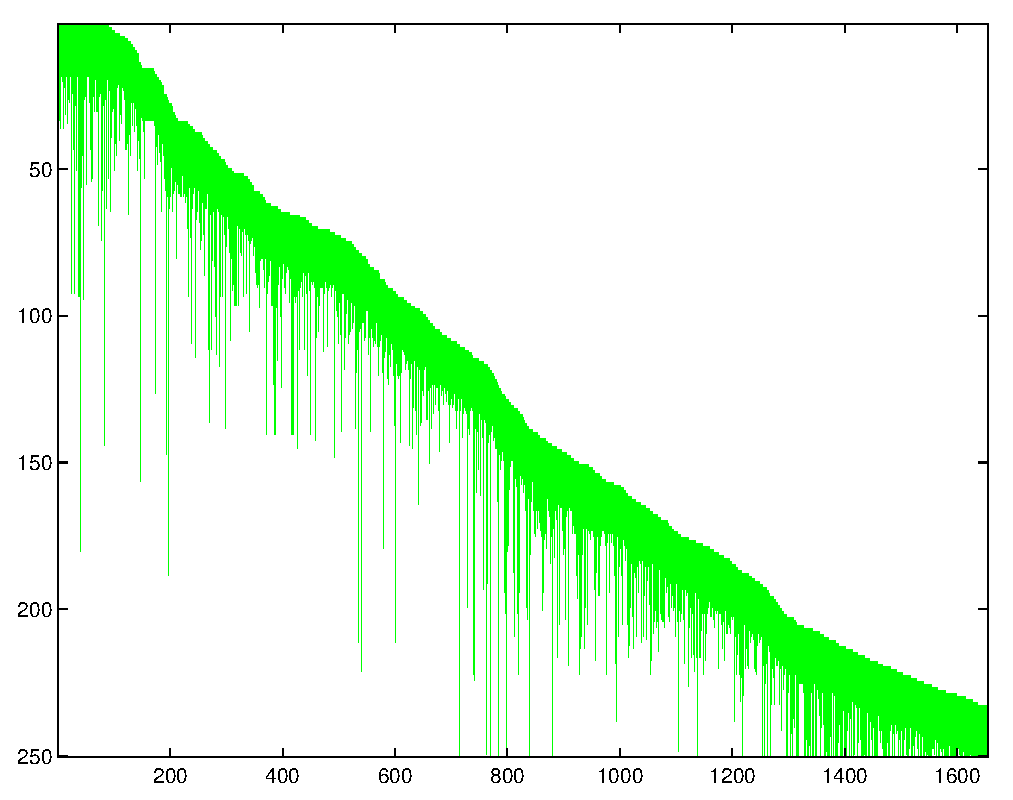
\includegraphics[width=0.7\textwidth,height=0.2\textwidth]{IMAGES/TroyW.eps} \\
 1768 tracks in 250 frames. Degree of visibility is about 14 \% 
\end{center}
\end{frame}



%-------------------------------------------------------------------
\begin{frame}
\frametitle{Affine projection}
Assume that the average depth is large compared to the depth
variation. Then the perspective projection may be approximated by  an
affine (orthographic) projection:
 
\begin{displaymath}
\left [ \begin{array}{c} x \\ y \end{array} \right ]
\;\;=\;\; 
\left [ \begin{array}{c c c} 
a_1 & a_2 & a_3 \\ b_1 & b_2 & b_3 
\end{array} \right ]
\; 
\left [ \begin{array}{c} X \\ Y \\ Z  \end{array} \right ] 
\;+\; 
\left [ \begin{array}{c} t_x \\ t_y  \end{array} \right ] 
\;\;=\;\; 
C \; 
\left [ \begin{array}{c} X \\ Y \\ Z  \end{array} \right ]
\;+\; {\bf t}
\end{displaymath}

The two vectors ${\bf a}$ and ${\bf b}$ may be seen as two first rows
os the camera matrix (The third is given by ${\bf a} \times {\bf b}$). \\[2mm]

Often we may assume that ${\bf a} \cdot {\bf b} = 0$ and that
$||{\bf a}|| \;=\; ||{\bf b}||$.

\end{frame}



%-------------------------------------------------------------------
\begin{frame}
\frametitle{The affine RSfM model}
If we stack all camera matrices $C_i$ into a $2N \times 3$ matrix $J$,
and let $K$ be a $3 \times M$ matrix of 3D coordinates of the $M$ 3D
points: \\

\begin{center}
\begin{displaymath}
  W \;=\; J \cdot K + {\bf t}
\end{displaymath}
\end{center}
where ${\bf t}$ is a $2N \times 1$ vector of translation values. \\[2mm]

It is easy to show that by subtracting the average row value from each
row (and redefining $J$) the model may be simplified:
\begin{center}
\begin{displaymath}
  W ::= (W - \bar{W}) \;=\; J \cdot K
\end{displaymath}
\end{center}
The row average subtraction correspond to centering all image
observation to their center of mass.

\end{frame}



%-------------------------------------------------------------------
\begin{frame}
\frametitle{The rank theorem}
The rank of a $n \times m$ matrix is the larges number of linearly
independent rows or columns (maximum of the row rank and the column
rank).  \\[3mm]

\begin{theo}
 The rank of the normalized measurement matrix is 3 
\end{theo}
$\mbox{}$\\[3mm]

The theorem directly follows by the construction of $W$ because both
$J$ and $K$ have rank 3.
\end{frame}




%-------------------------------------------------------------------
% \begin{frame}
% \frametitle{Matrix factorization}
% Matrices may be factorized (into products of other matrices) in a
% number of ways: \\[3mm]
% \begin{itemize}
%  \item LU-decomposition
%  \item Eigenvalue decomposition
%  \item QR-decomposition
%  \item SVD-decomposition \\[3mm]
% \end{itemize}
% You are not suposed to know these, nor their advantages etc, but they
% are really useful.  Here we will use the Singular Value Decomposition (SVD).
% \end{frame}



%-------------------------------------------------------------------
% \begin{frame}
% \frametitle{SVD}
% Any matrix $A$ may be decomposed into a product of 3 matrices:
%
% \begin{center}
% \begin{displaymath}
%   A \;\;=\;\; U \; D \; V^{\top}
% \end{displaymath}
%\end{center}
%
% where $U$ is a column orthonormal matrix, $D$ is a diagonal matrix
% with positive values, and $V$ is a unitary matrix:
%
% \begin{center}
% \begin{eqnarray*}
%  U^{\top} U & = & I \\
%  V^{\top} V & = & V V^{\top} \; = \; I
% \end{eqnarray*}
% \end{center}
%
% The singular values in the diagonal of $D$ are usually sorted in
% decreasing order.  If we zero out all but the 3 largest and recompute:
%
% \begin{center}
% \begin{displaymath}
%   \hat{A} \;\;=\;\; U \; D_3 \; V^{\top}
% \end{displaymath}
% \end{center}
% 
% we get a matrix $\hat{A}$ of rank 3 and as close to $A$ as possible.
% \end{frame}



%-------------------------------------------------------------------
\begin{frame}
\frametitle{How to obtain the factorization}
Apply SVD and zero out all but the 3 largest singular values.
\begin{center}
\begin{displaymath}
  \hat{W} \;\;=\;\; U_3 \; D_3 \; V_3^{\top}
\end{displaymath}
\end{center}
where $U_3$ is the first 3 columns of $U$, $V_3$ is the first 3
columns of $V$, and $D_3$ is the upper left $3 \times 3$ submatrix of
$D$. 

\begin{center}
   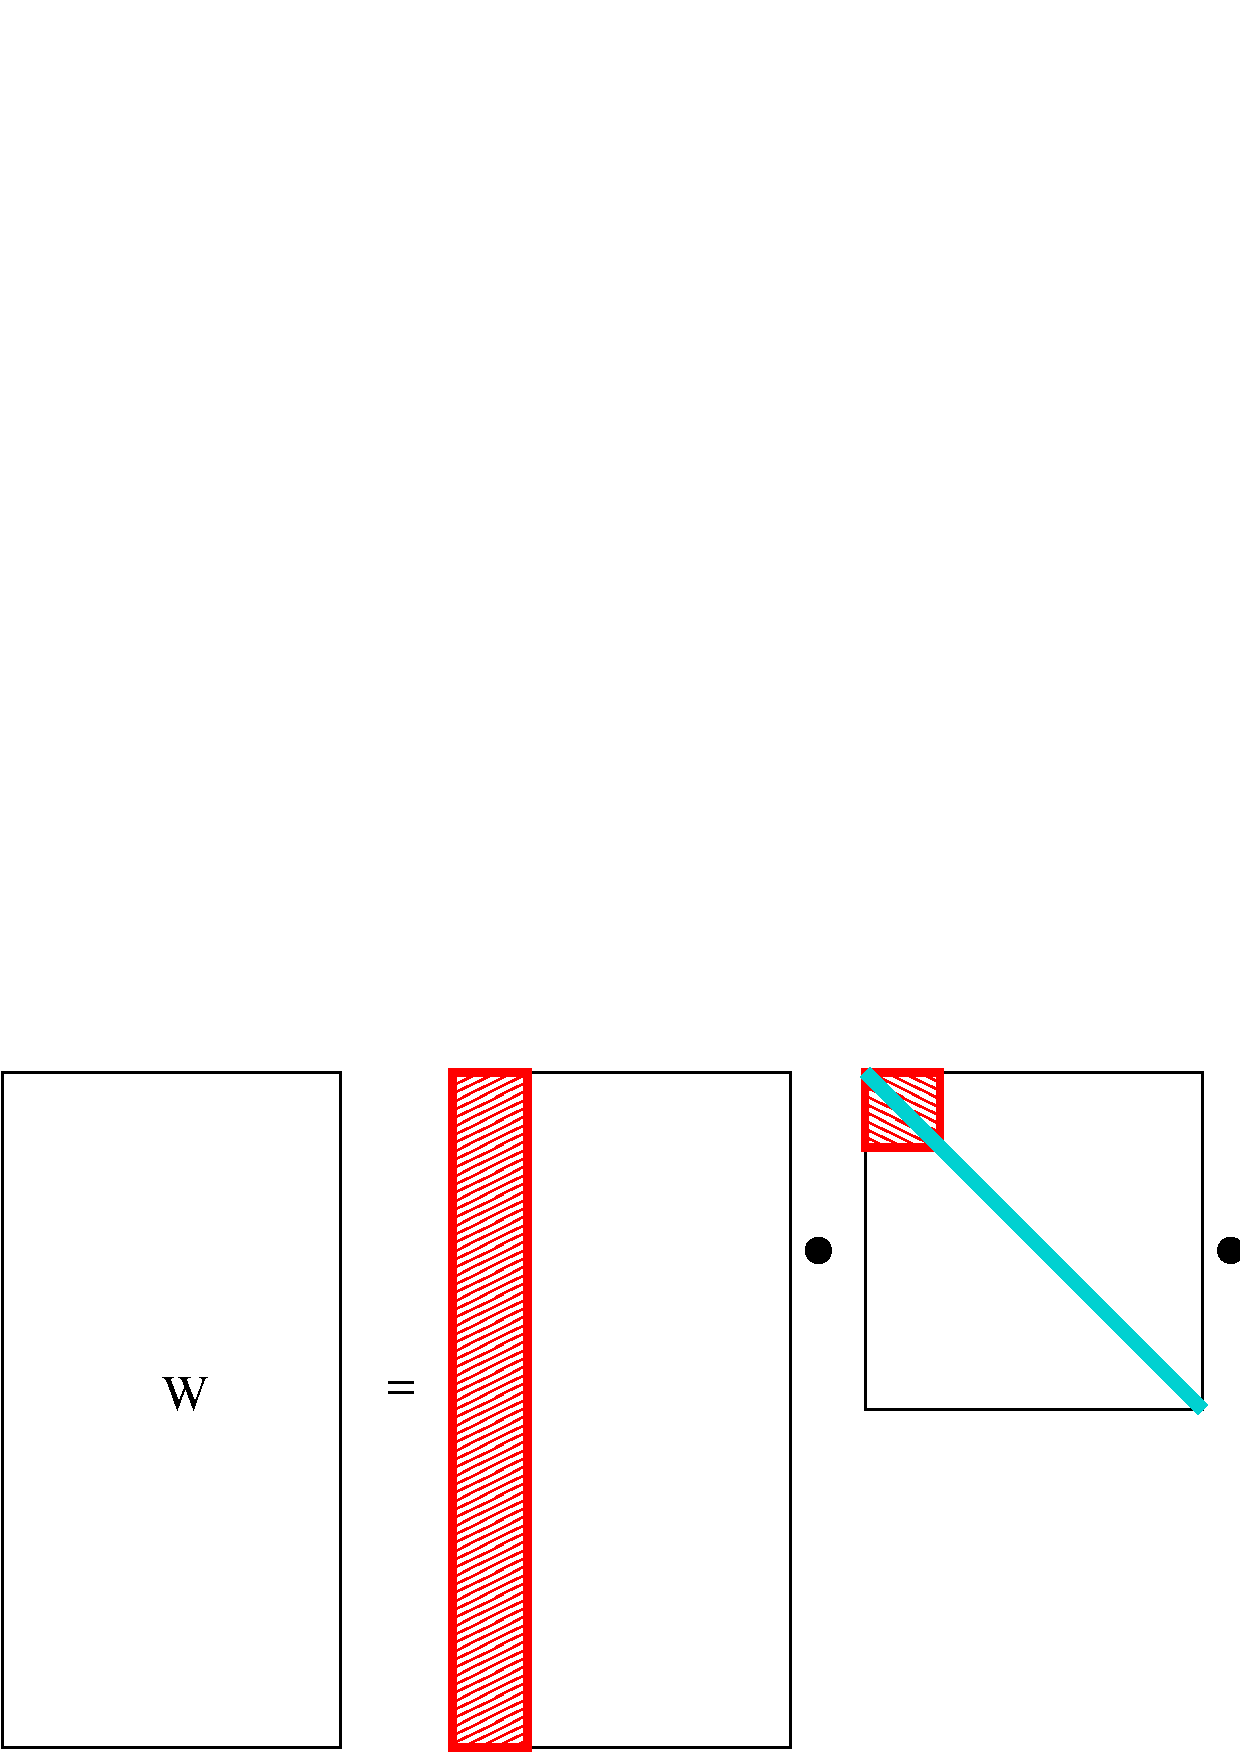
\includegraphics[width=0.8\textwidth]{MyImages/factor.jpg}
\end{center}

\end{frame}



%-------------------------------------------------------------------
\begin{frame}
\frametitle{How to split the factorization}
The square root $\sqrt{D}$ of a diagonal matrix $D$ is a diagonal
matrix with the square root of the diagonal values. \\[3mm]

Given the normalized measurement matrix $W$ we factorize using:
\begin{center}
\begin{displaymath}
  \hat{W} \;\;=\;\; (U_3 \; \sqrt{D_3}) \;\; (\sqrt{D_3} \; V_3^{\top})
   \;\;=\;\; J \; K  
\end{displaymath}
\end{center}
We also see that if $Q$ is a full rank $3 \times 3$ mixing matrix,
that specifies the coordinate frame in which the cameras (and 3D
points) are reconstructed, then:

\begin{displaymath}
  \hat{W} \;\;=\;\; J \; K  \;\;\;=\;\; J Q \; Q^{-1} \; K 
\end{displaymath}
  
We must specify $Q$ to get the reconstruction in a right-angled
coordinate system.
\end{frame}



%-------------------------------------------------------------------
\begin{frame}
\frametitle{The mixing matrix}
To fix the mixing matrix $Q$, we consider the $2 \times 3$ submatrices
$J_i$.  We would like $Q$ to transform this into the form  
$A_i R_i$, where $R_i$ contains the first 2 rows of the camera
rotation matrix and $A_i$ contains the internal camera parameters.
Thus:

\begin{center}
\begin{displaymath}
  J_i  Q  \;=\;  A_i  R_i
\end{displaymath}
\end{center}

Now multiply each side with its transpose:
\begin{center}
\begin{displaymath}
  J_i Q  Q^{\top}  J_i^{\top}   \;=\; 
  A_i R_i  R_i^{\top}  A_i^{\top}  \;=\; 
  A_i A_i^{\top}  
\end{displaymath}
\end{center}
\end{frame}


%-------------------------------------------------------------------
\begin{frame}
We now assume that the aspect ratio is 1 (pixels are square) and that
the coordinate axes are perpendicular.  Leaving open the question on
scaling, i.e.:
\begin{center}
\begin{displaymath}
  \hat{W} \;\;=\;\;  J \; K  \;\;=\;\; (k J) (\frac{1}{k} K)
\end{displaymath}
\end{center}

we see that:
\begin{center}
\begin{displaymath}
A_i A_i^{\top}  = I
\end{displaymath}
\end{center}

We now have ($\forall i$):
\begin{center}
\begin{displaymath}
  J_i Q  Q^{\top}  J_i^{\top}   \;=\;  J_i X  J_i^{\top}   \;=\; I
\end{displaymath}
\end{center}

where $X = Q Q^{\top}$.  
\end{frame}




%-------------------------------------------------------------------
\begin{frame}
We may write out the set of linear equations in $X$ using the
partition of $J_i$ into row vectors ${\bf a}$ and ${\bf b}$.
\begin{center}
\begin{displaymath}
J_i \;=\; \left ( 
\begin{array}{c} {\bf a}_i^{\top} \\ {\bf b}_i^{\top} \end{array}
\right )
\end{displaymath}
\end{center}

It is easy to check that the conditions for the mixing matrix $Q$ is $\forall i$:
\begin{eqnarray*}
a_i^{\top} X a_i   &  = & 1 \\ 
a_i^{\top} X b_i    &  = & 0 \\
b_i^{\top} X b_i     &  = & 1 
\end{eqnarray*}
where $X = Q Q^{\top}$. \\[3mm]

Although the first set of $3N$ equations are linear the last
matrix-equation is not.  Thus, we need non-linear optimization
(e.g.  {\em lsqnonlin} in MATLAB) to find the solution.
\end{frame}





%-------------------------------------------------------------------
\begin{frame}
\frametitle{Tomasi-Kanade factorization -- Opsumering}
  \begin{itemize}
  \item Identify/match tracks and construct the measurement matrix
    $W$. Then normalize by subtracting the row-average value. \\[3mm]
  \item Factorize $W =U D V^{\top}$. Zero out all but 3 largest
    singular values and construct $J$ and $K$ \\[3mm]
  \item Solve for the mixing matrix $Q$ \\[3mm]
  \item Compute $JQ$ and $Q^{-1}K = S$ \\[3mm]
  \item Use 3D shape points $S$ to whatever needed  
  \end{itemize}
\end{frame}




%-------------------------------------------------------------------
\begin{frame}
\begin{center}
   \includegraphics[width=\textwidth]{IMAGES/Colosseum.jpg}
\end{center}

\end{frame}




%-------------------------------------------------------------------
\begin{frame}
\frametitle{Extensions to Tomasi-Kanade}
It is possible to generalize the approach: \\[3mm]

\begin{itemize}
  \item To use perspective projection
  \item To hande outliers (false matches)
  \item To handle partial data
  \item To model deforming (non-rigid) objects \\[3mm]
\end{itemize}

This is all too advanced for this this course.  One entry-point is: \\
S. I. Olsen and A. Bartoli:
{\em  Implicit Non-Rigid Structure-from-Motion with Priors},
Journal of Mathematical Imaging and Vision, Vol. 31, no.2-3, 
pp. 233-244, 2008.
\end{frame}


% describe how block-processing may be used


% See Adriens slides in ~/teaching/DATAMATSYN/ABslides/Lecture2.{3-5}.pdf
% coordinate frame ambiguity
% 



\begin{frame}
\frametitle{End of lectures}

\begin{itemize}
  \item Questions for today ?
  \item Questions for the course ?
  \item Other questions, comments, ... ? \\[8mm]
\end{itemize}

\pause
{\large
\color{blue}{You have already evaluated the course on KU-net. For
  improving the course this evaluation is not useful. \\[4mm]

Now we will like to hear more specific comments from you}
}
\end{frame}





%-------------------------------------------------------------------
% \begin{frame}
% \frametitle{Evaluation}
%
% {\bf Remember the course description:} \\
% {\Large
% \begin{quote}
% {\color{blue}{The objective is to provide students with a general
%    introduction to visual cognitive models and its relevance to
%    modern image processing. The course also provides students with
%    the necessary mathematical background to understand vision and
%    image processing methods and includes programming exercises.}} 
% \end{quote}
% }
% \end{frame}



%-------------------------------------------------------------------
\begin{frame}

{\bf \color{blue}{You are supposed to have learned:}}
  \begin{itemize}
  \item Theoretical and practical knowledge of the
    current research within computer vision and image analysis. \\[3mm]
  \item Knowledge of common application areas. \\[3mm]
  \item To read and apply the knowledge obtained by reading scientific
    papers.  \\[3mm]
  \item To convert a theoretical algorithmic description into a
    concrete program implementation.  \\[3mm]
  \item  To compare computer vision and image analysis algorithms and
     assess their ability to solve a specific task. \\[3mm]
  \item To understand and analyze the main challenges in vision and
    image processing today \\[3mm]
  \end{itemize}


{\color{blue}{Think a little if you have achieved the learning goals
    and if there was elements in the course or in the teaching that
    was particular good or bad}}  
\end{frame}


% -------------------------------------------------------------------
\begin{frame}
\frametitle{Possible points of interest}

\begin{enumerate}
   \item The reading material
   \item The assignments (readability, difficulty, ...)
   \item The lectures 
   \item The exercises (did you receive help)
   \item The course content
   \item The usability
\end{enumerate}
\end{frame}


% -------------------------------------------------------------------
\begin{frame}
\frametitle{Class evaluation}

\begin{enumerate}
   \item{\color{red}{Write 3 short statements}} (1-3 lines) about
     good and/or bad elements of the course on a A4-page.  Leave space
     between the statements. 
   \item Repeat until you get your own statements back
   \begin{enumerate}
      \item Pass on your statemensts to your right neighbor and
        receive a page with statements from your left neighbor.
      \item For each statement on each page (excluding your own):
      \begin{itemize}
         \item {\color{red}{Put a dash if you agree on the
               statement}}. Otherwise don't put a dash.
      \end{itemize}
  \end{enumerate}
  \item Let N = number of statement with most votes
  \item For i = N to N-5
  \begin{itemize}  
     \item Read out loud the statement and write it on the backboard
     \item Ask for supplementary comments from all
  \end{itemize}
  \item Ask if any have a really important statement that did not
    receive many votes, but has to be mentioned.
\end{enumerate}

\end{frame}

\end{document}


